% !Mode:: "TeX:UTF-8"
%!TEX program  = xelatex

%\documentclass{cumcmthesis}
\documentclass[withoutpreface,bwprint]{cumcmthesis} %去掉封面与编号页
%\documentclass[UTF8]{ctexart} 
%\setlength\parindent{2em}
%\usepackage{SIunits}
\usepackage{url}
\usepackage{array}
\usepackage{amsmath} 
\usepackage{amssymb}
\usepackage{amsfonts}
\usepackage{caption}
\usepackage{booktabs}
\usepackage{color}
\usepackage{enumerate}
\usepackage{xpatch}
\usepackage{graphicx}
\usepackage{longtable}
\usepackage{multirow}
\usepackage{comment}
\usepackage{subfigure}
\usepackage{supertabular}
\usepackage{floatrow}
\usepackage{cite}
\usepackage{float}
\usepackage{ctex}
\usepackage{bm}

\xpatchcmd{\thebibliography}{\section*}{\section}{}{}
%\newcommand{\upcite}[1]{\textsuperscript{\textsuperscript{\cite{#1}}}}

\title{高压油管的压力控制}
\tihao{A}
\baominghao{201922002029}
\schoolname{重庆邮电大学}
\membera{陈恒宇}
\memberb{邓韦}
\memberc{殷寰宇}
\supervisor{虞继敏}
\yearinput{2019}
\monthinput{09}
\dayinput{15}


\begin{document}
\maketitle
\begin{abstract}
        本文通过

        针对问题一,
        
        针对问题二,
        
        针对问题三,
        
        
\keywords{关键词}
\end{abstract}
%\thispagestyle{empty}

%目录
%\tableofcontents
%\thispagestyle{empty}

%\newpage

\section{问题重述}
\subsection{问题背景}
        燃油发动机使燃料燃烧并产生动力,是驱动汽车各部分正常工作或行驶的保障。                      
    而燃油进入和喷出高压油管是燃油发动机工作的基础,其进入和喷出的过程会导致
    高压油管内压力的变化,进而导致喷嘴喷油量的偏差,从而影响发动机的工作效率。
    因此,通过理论分析和计算,给出合理的高压油管控制方案对发动机高效工作有着
    积极影响。

\subsection{问题的提出}
        燃油经高压油泵进入油管,再由喷口喷出。
    %燃油压力变化量与密度变化量之比为$\frac{E}{\rho}$,其中$\rho$为燃油密度,$E$为杨氏模量,其与压力的关系
    %见附件3。
    根据高压油管工作原理(图\ref{figure1}),
    回答以下问题:

(1)已知高压油管尺寸、初始压力及喷油嘴工作次数和工作时间,设高压油泵在入口A
    处提供160MPa稳定压力,为使管内压力尽可能稳定在100MPa不变,应如何设置
    单向阀每次开启时长?若经过2s、5s和10s的调整后,管内压力从100MPa增加到
    150MPa并稳定,又应如何调整开启时长?
    %设高压油管内腔长500mm,直径10mm,供油入口处有一直径1.4mm的小孔,且由
    %单向阀控制供油时间长短,每次打开后都需关闭10ms才能再一次开启。喷油嘴每
    %秒工作10次,每次喷油2.4ms。油管内
    %初始压力为100MPa,若

(2)若高压油管入口处燃油来自油泵的柱塞腔出口,柱塞运动由凸轮驱动,喷油由油嘴
    的针阀控制。已知各部分的工作原理和相关参数,在问题1喷油器工作次数、高压
    油管尺寸和初始压力下,确定凸轮工作的角速度,使得油管内压力尽可能稳定在
    100MPa。

(3)在问题2的基础上增加一个相同的喷油嘴,应如何调整喷油和供油策略?若安装
    单向减压阀来更好地控制油管压力,请给出油泵和减压阀的控制方案。

\begin{figure}[!h]
    \centering
    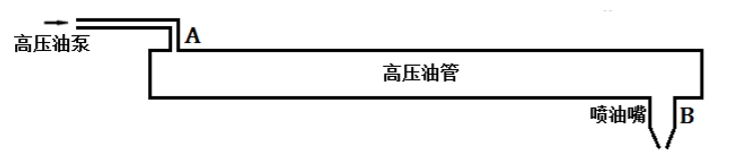
\includegraphics[width=.8\textwidth]{figure1.png}
    \caption{高压油管工作原理示意图}
    \label{figure1}
\end{figure}

\section{问题分析}
\subsection{问题一的分析}   


\subsection{问题二的分析}
        

\subsection{问题三的分析}
        
     

\section{基本假设}
(1)假设高压油管与油泵内的气体均为理想气体,且压缩、膨胀过程中无温度变化。

(2)假设供给和喷出燃油的过程中油管与油泵内气体与外界气体均无交换。    

\section{符号说明}
\begin{center}
\begin{tabular}{ccc}
%\caption[table]{符号说明}
\toprule[2pt]
\makebox[0.2\textwidth][c]{符号}&\makebox[0.5\textwidth][c]{意义}&\makebox[0.2\textwidth][c]{单位} \\
\midrule[1pt]
 $R_i$  &  第$i$个雷达  & / \\ 
 $r_i$  &  飞行物与第$i$个雷达之间距离的观测值  &  米  \\ 
 $(x_i,y_i,z_i)$  &  第$i$个雷达的坐标  &  米  \\ %\hline
 $S(x,y,z)$  &  飞行物坐标  &  米  \\% \hline
 $N$  &  飞行物乙的$x$轴坐标  &  公里 \\ %\hline
 $M$  &  安全区的$y$轴坐标  &  公里  \\
 $h$  &  飞行物乙的$z$轴坐标  &  公里  \\
 $V$  &  敌机的飞行速度  &  马赫数  \\
 $U$  &  I型追踪导弹的速度  &  马赫数  \\
 $V_{\text{声}}$  &  测量地的音速  &  米/秒  \\
 $n$  &  雷达的个数  &  个  \\
\bottomrule[1.5pt]
\end{tabular}
\end{center}

\section{问题一的求解}
\subsection{高压油管内的压力}
    因燃油的压力变化量与密度变化量成正比,且比例系数为$\frac{E}{\rho}$,可以得到
    燃油密度的计算公式
    \begin{equation}
        \frac{\triangle P}{\triangle \rho}=\frac{E}{\rho}
    \label{equ1}
    \end{equation}
    其中,$P$为当前压力,$\rho$为燃油密度,$E$为弹性模量,且其与压力的关系如附件3
    所示。设初始压力$P_0=100~MPa$,此时燃油密度$\rho_0=0.850~mg/mm^3$,
    则$\triangle P=P-P_0$,$\triangle \rho=\rho-\rho_0$,带入公式(\ref{equ1})
    中可得
    \begin{equation}
        \frac{P-P_0}{\rho-\rho_0}=\frac{E}{\rho}
    \label{equ2}
    \end{equation}    
    整理得
    \begin{equation}
        \rho=\frac{\rho_0}{1-\frac{P-P_0}{E}}
    \label{equ3}
    \end{equation}    
   
    
    设高压侧燃油密度为$\rho$,流量系数$C=0.85$,小孔面积$A=\pi r_{A}^2$,
    油泵在入口$A$处的压力$P_1=160~MPa$,小孔$A$两端的压力差$\triangle P=P_1-P$。
    则单位时间内经小孔$A$流入高压油管的燃油量为
    \begin{equation}
        Q=CA\sqrt{\frac{2\triangle P}{\rho}}=CA\sqrt{\frac{2(P_1-P)}{\rho}}
    \label{equ4}
    \end{equation}    
    将$P=160~MPa$带入公式(\ref{equ3})中,求得$\rho=0.8687$。

    假设高压油管内的气体为理想气体,且体积压缩和膨胀过程中无温度变化,
    则其压强与体积满足波义尔定律$P_0V_0=PV$。
    其中,$V_0$为高压油管内腔总体积,$P_0$为油管初始压力
    $100~MPa$。设$t$时刻进入油管的燃油量为$q$,排出量为$e$,则管内体积变化量
    \begin{equation}
        \triangle V=V_{\text{进入}}-V_{\text{喷出}}=\int_0^t q dt-\int_0^t e dt
    \label{equ5}
    \end{equation}
    $t$时刻高压油管内的压力$P=P_0V_0 / V$,气体体积$V=V_0-\triangle V$,
    代入公式(\ref{equ5})可以求得
    \begin{equation}
        P=\frac{P_0V_0}{V_0-\int_0^t q dt+\int_0^t e dt}
    \label{equ6}
    \end{equation}

\subsection{单目标优化模型}
    因高压油管内腔长$L_{\text{油管}}=500~mm$,内直径$d_{\text{油管}}=10~mm$,
    入口$A$的直径$d_A=1.4~mm$,则
    $V_0=\pi (d_{\text{油管}}/2)^2\cdot L_{\text{油管}}=12500\pi ~mm^3$,
    $A=\pi (d_A/2)^2=0.49\pi ~mm^2$。
    已知小孔A通过单向阀开关控制供油时间,且每次打开后就要关闭$10~ms$,设每次开启
    时间为$t_{\text{开}}$,则单向阀工作周期$T=(t_{\text{开}} + 10)~ms$;
    喷油器每秒工作10次,每次喷油$2.4~ms$且喷油速率如图\ref{figure2}所示。
    \begin{figure}[htbp]
        \centering
        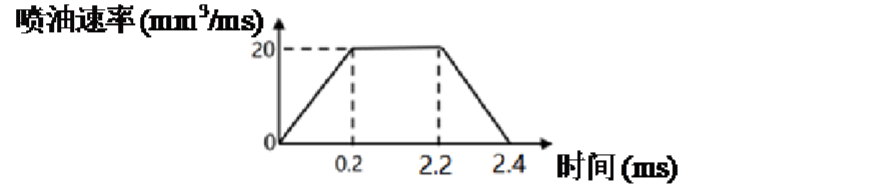
\includegraphics[width=.7\textwidth]{E_rate.png}
        \caption{喷油速率示意图}
        \label{figure2}
    \end{figure} \\
    则$t$时刻喷油量
    \begin{eqnarray}
    e=
    \begin{cases}
        100t \quad \quad \quad & 0 \leq t \leq 0.2 \\
        20   & 0.2 < t \leq 2.2 \\
        240-100t  & 2.2 < t \leq 2.4 \\
        0 & 2.4 < t <100
    \end{cases}
    \label{equ7}
    \end{eqnarray}

    由公式(\ref{equ4})可知,进入油管的燃油量$q$为$P$的函数({\color{red}这里有点问题}),
    将$q$和$e$代入公式(\ref{equ6})中进行求解即可得到油管内压力$P$与时间$t$的方程。
    因该方程过于复杂无法直接求解,故采用如下方法计算:
    
    \textbf{Step1}:将时间段$[0,t]$分割为若干个长度为$\triangle t=0.01~ms$的小区间,
    第$i$个区间内燃油的进入和喷出量分别记为$\triangle q_i$和 $\triangle e_i$
    $(i=1,2,\cdots,n)$。

    \textbf{Step2}:在第$i$个区间上以起始点的$q_i$与$e_i$的值近似代替连续变化的值,即
    \begin{eqnarray}
        \begin{cases}
            \triangle q_i \approx q_i\triangle t\\
            \triangle e_i \approx e_i\triangle t
        \end{cases}
        %,\quad \quad  i=1,2,\cdots,n \quad \text{且} \quad
        %n=\lfloor{\frac{t}{\triangle t}}\rfloor
    \label{equ8}
    \end{eqnarray}
    其中$i=1,2,\cdots,n$且$n=\lfloor{\frac{t}{\triangle t}}\rfloor$。
    
    \textbf{Step3}:求$n$个时间段进入和喷出燃油量的和,即
    \begin{eqnarray}
        \begin{cases}
            V_{\text{进入}}=\int_0^t q dt \approx
             \sum\limits_{i=1}^n \triangle q_i \\
            %=\sum\limits_{i=1}^n q_i\triangle t \\
            V_{\text{喷出}}=\int_0^t e dt \approx
             \sum\limits_{i=1}^n \triangle e_i \\
            %=\sum\limits_{i=1}^n e_i\triangle t
        \end{cases}
    \label{equ9}
    \end{eqnarray}

    \textbf{Step4}:记第$i$个区间起始时刻压强为$P_{i-1}$,结束时刻压强为$P_i$,则
    \begin{eqnarray}
        q_i=
        \begin{cases}
        CA\sqrt{\frac{2(P_1-P_{i-1})}{\rho}} \quad \quad  \quad
        & i-\lfloor{\frac{t}{T}}\rfloor \cdot T \leq t_{\text{开}}\\
        0 & t_{\text{开}} < i-\lfloor{\frac{t}{T}}\rfloor \cdot T < T
        \end{cases}
    \label{equ10}
    \end{eqnarray}

    \textbf{Step5}:将公式(\ref{equ7}-\ref{equ10})依次代入公式(\ref{equ6})中
    可得关于压力的递推关系式
    \begin{equation}
        P_i=\frac{P_0V_0}
        {V_0-\sum\limits_{i=1}^n CA\sqrt{\frac{2(P_1-P_{i-1})}{\rho}}\cdot\triangle t +\sum\limits_{i=1}^n e_i\triangle t}
    \label{equ11}
    \end{equation}
    通过公式(\ref{equ11})不断迭代即可得到$[0,t]$时间段内各区间对应的压强。

    本题首先要求将高压油管内的压力尽可能稳定在$100~MPa$左右,令
    \begin{equation}
        F(t_{\text{开}})=\sum\limits_{i=1}^n (P_i-100)^2
    \label{equ12}
    \end{equation}
    其中,
    $n=\lfloor{\frac{t}{\triangle t}}\rfloor$,$t=1000~ms$。
    故单向阀每次开启时长的最优设置方案为各时刻压力与$100~MPa$距离的平方和
    $F(t_{\text{开}})$最小时。由此建立单目标优化模型,目标函数为
    \begin{equation}
       min \quad F(t_{\text{开}})
    \label{equ13}
    \end{equation}

    为求解上述问题的近似全局最优解,采用模拟退火算法,具体步骤如下:

    \textbf{Step1}:初始化目标函数值$F(t_{\text{开}})=0$,设置退火起点
    $t_{\text{开}}=0$,降温系数$\alpha=0.999$,终止温度$T^n=10^{-30}$,
    当前时间为$T_1$。

    \textbf{Step2}:对当前开启时间$t_{\text{开}}$进行变换得到新解$t_{\text{开}}'$,并带入目标
    函数中求出函数值。

    \textbf{Step3}:计算增量$\triangle F=F(t_{\text{开}}')-t_{\text{开}}$。
    
    \textbf{Step4}:若$\triangle F<0$,则将$t_{\text{开}}'$作为新的当前解,
    否则以概率$exp(-\triangle F/T_1)$接受$t_{\text{开}}'$作为当前解。

    \textbf{Step5}:当$T_1 \leq ^n$时,退火算法结束,当前解即近似全局最优解;
    否则返回Step2。

\subsection{油管压力稳定在$100MPa$的控制方案}
    用MATLAB求解5.2中的单目标优化模型,得到单向阀每次开启时间的最优解为
    $t_{\text{开}}=0.314~ms$,$F(0.314~ms)=173.27$。
    代入公式(\ref{equ11})后作压力随时间变化的图像。 
    \begin{figure}[!h]
    \centering
    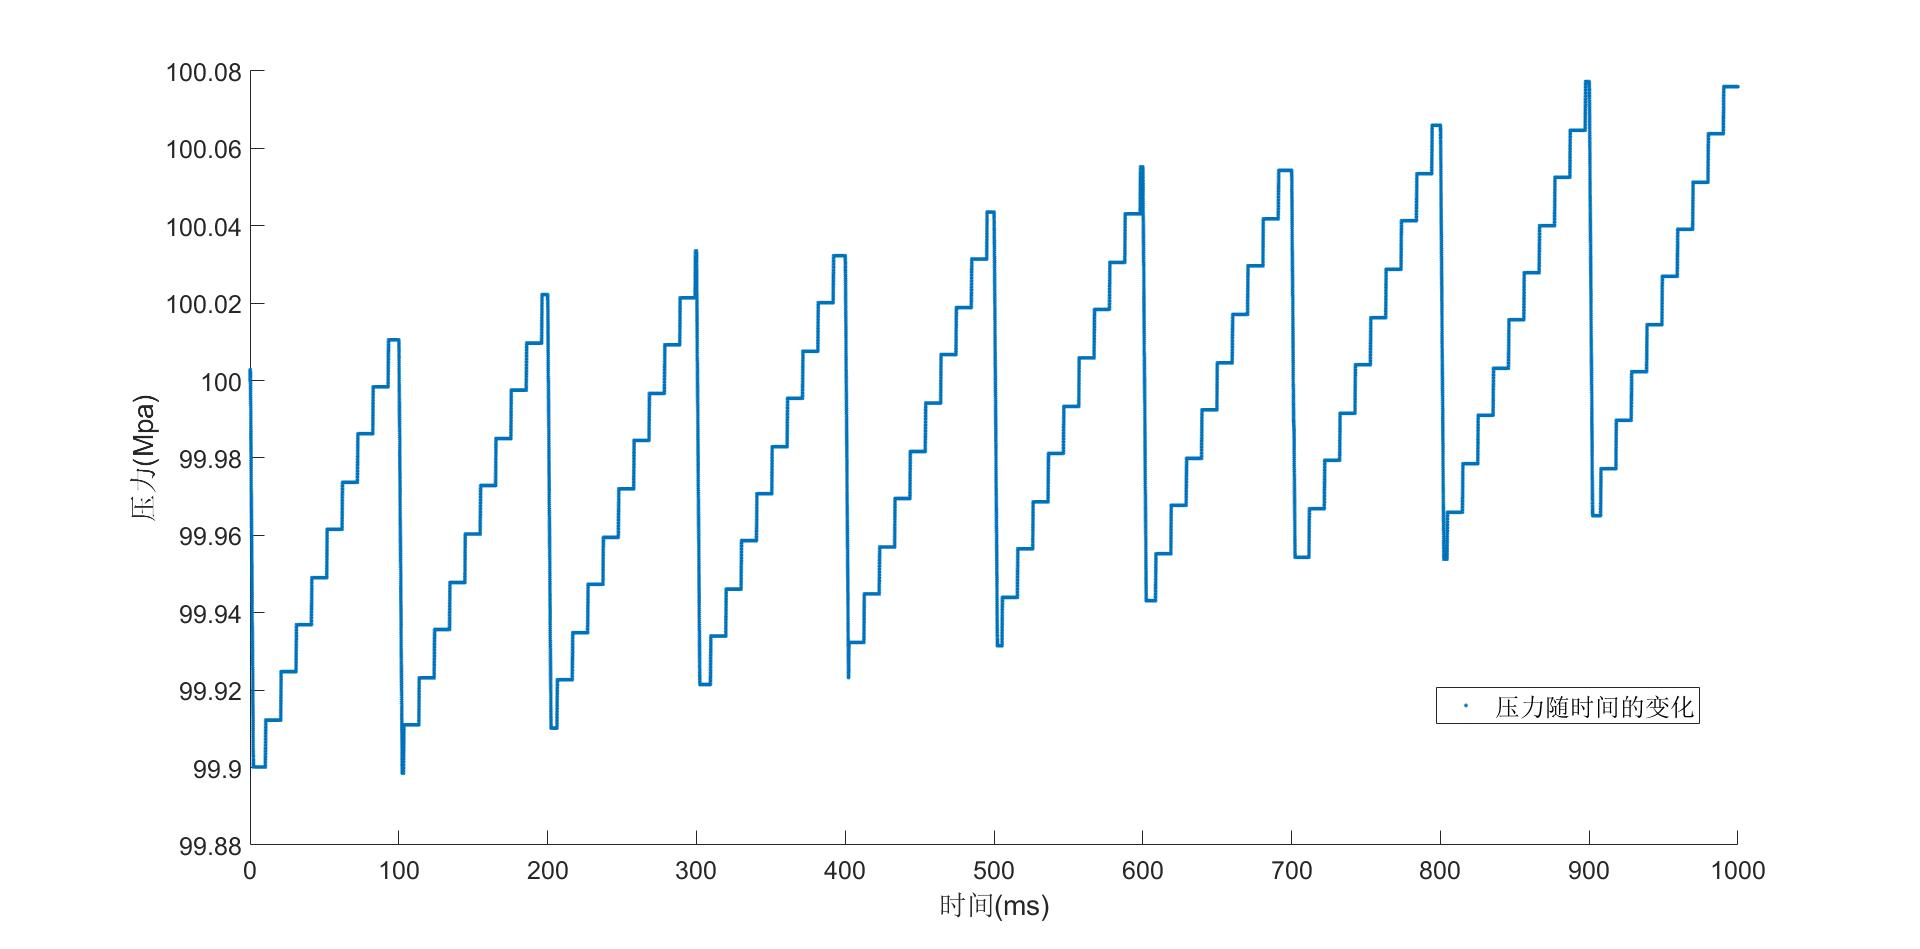
\includegraphics[width=.95\textwidth]{100Mpa.jpg}
    \caption{稳定在$100~MPa$时压力随时间变化示意图}
    \label{figure3}
    \end{figure}

    由图\ref{figure3}可以看出$1s$内高压油管的压力在$100~MPa$上下小幅度波动,
    且100000个区间的平均偏离量仅为$1.7327e-3$,说明压力较为稳定。

\subsection{油管压力增加到在$150MP$a的调整方法}


\section{问题二的求解}

\subsection{模型的建立与求解}


\section{问题三的求解}

\subsection{模型的建立与求解}



\section{灵敏度检验}

\section{模型的评价}
\subsection{模型的评价}
\subsubsection{模型的优点}

\subsubsection{模型的缺点}

\section{模型的改进}
1、传感器

2、流量系数
   

%参考文献
\begin{thebibliography}{9}%宽度9
\bibitem{bib:one}曾文军,曾小雨,郑娟,朱金伟.
    多雷达定位误差简析[J].高等函授学报(自然科学版),
    2008(05):57-59.
\bibitem{bib:two}

\end{thebibliography}


\newpage
%附录
\begin{appendices}
\section{引用}
  问题一要求我们根据CMA热带气旋最佳路径数据集和{\bfseries\heiti 其他相关资料},
对中国各省(以地级市为单位){\cu 进行}进行热带气旋的风险评估。
首先统计出1949年-2018年登录我国沿海各省份的热带气旋数量,
并选取其中登录次数 最多的四个省份作为评估对象。
{\bfseries 其次确定}评定热带气旋风险等级的八个因素:{\cu 受热带气旋}影响过程中的
平均降雨量、{\chu 日最大}降雨量、平均风速、日最低气压、热带气旋的登陆频次、持续时间、
造成的人员伤亡数和直接经济损失。
接着确定四个热带气旋风险等级分别为:灾情较轻,灾情一般,灾情较重,灾情严重。
由于对热带气旋风险的评估属于模糊决策,故采用模糊综合评价法求出各省受热带气旋
影响的评价结果。\cite{bib:one}
最后在四个受灾最严重的省份中各选取四个典型城市,采用相同的方法进行风险评估,
并结合地理、气候因素分析其对风险等级的影响。

\section{排队算法--matlab 源程序}
    \begin{lstlisting}[language=matlab]
    kk=2;[mdd,ndd]=size(dd);
    while ~isempty(V)
    [tmpd,j]=min(W(i,V));tmpj=V(j);
    for k=2:ndd
    [tmp1,jj]=min(dd(1,k)+W(dd(2,k),V));
    tmp2=V(jj);tt(k-1,:)=[tmp1,tmp2,jj];
    end
    tmp=[tmpd,tmpj,j;tt];[tmp3,tmp4]=min(tmp(:,1));
    if tmp3==tmpd, ss(1:2,kk)=[i;tmp(tmp4,2)];
    else,tmp5=find(ss(:,tmp4)~=0);tmp6=length(tmp5);
    if dd(2,tmp4)==ss(tmp6,tmp4)
    ss(1:tmp6+1,kk)=[ss(tmp5,tmp4);tmp(tmp4,2)];
    else, ss(1:3,kk)=[i;dd(2,tmp4);tmp(tmp4,2)];
    end;end
    dd=[dd,[tmp3;tmp(tmp4,2)]];V(tmp(tmp4,3))=[];
    [mdd,ndd]=size(dd);kk=kk+1;
    end; S=ss; D=dd(1,:);
    \end{lstlisting}

\section{长表格}
\begin{longtable}[c]{p{0.2\textwidth}<{\centering}|p{0.1\textwidth}<{\centering}p{0.2\textwidth}<{\centering}}
    %\centering
    \caption{abcd} \\
    \toprule[2pt]
    增益介质&功率& 波长\\ 
    \midrule[1pt]
    \endfirsthead
    \caption[]{abcd(绪)} \\
    %\multicolumn{3}{r}{\footnotesize 接上页} \\ 
    \toprule[2pt]
    增益介质&功率&波长\\ 
    \midrule[1pt]
    \endhead
    \bottomrule[1.5pt] 
    %\multicolumn{3}{r}{\footnotesize 接下页} \\
    \endfoot
    \bottomrule[1.5pt]
    \endlastfoot
    HeNe & \multicolumn{2}{c}{000} \\
    HeNe & 1mW & 633nm \\\cline{1-2} 
    %纵向合并
    \multirow{2}{0.2\textwidth}{\centering000}
     & 1mW & 633nm \\
     & 1mW & 633nm \\
    HeNe & 1mW & 633nm \\
    HeNe & 1mW & 633nm \\
    HeNe & 1mW &  633nm \\
    HeNe & 1mW & 633nm \\
    HeNe & 1mW & 633nm \\
    HeNe & 1mW & 633nm \\
    HeNe & 1mW & 633nm \\
    HeNe & 1mW & 633nm \\
    HeNe & 1mW & 633nm \\
    HeNe & 1mW & 633nm \\
    HeNe & 1mW & 633nm \\
    HeNe & 1mW & 633nm \\
    HeNe & 1mW & 633nm \\
    HeNe & 1mW & 633nm \\
    HeNe & 1mW & 633nm \\
    HeNe & 1mW & 633nm \\
    HeNe & 1mW & 633nm \\
    HeNe & 1mW & 633nm \\
    HeNe & 1mW & 633nm \\
    HeNe & 1mW & 633nm \\
    HeNe & 1mW & 633nm \\
    HeNe & 1mW & 633nm \\
    HeNe & 1mW & 633nm \\
    HeNe & 1mW & 633nm \\
    HeNe & 1mW & 633nm \\
    HeNe & 1mW & 633nm \\
    HeNe & 1mW & 633nm \\
    HeNe & 1mW & 633nm \\
    HeNe & 1mW & 633nm \\
    HeNe & 1mW & 633nm \\
\end{longtable}

\section{表格}
\begin{table}[htbp]
    \caption{风险评估对象(地级市)}
    \centering    
    \label{table1}
    \begin{tabular}{m{0.1\textwidth}<{\centering}|
        m{0.1\textwidth}<{\centering}m{0.1\textwidth}<{\centering}
        m{0.1\textwidth}<{\centering}m{0.1\textwidth}<{\centering}}
    \toprule[2pt]
         省份  &  \multicolumn{4}{c}{城市}  \\%横向合并
    \midrule[1pt]
        浙江  &  杭州  &  湖州  &  金华  &  丽水  \\
        \cline{1-3}
        %纵向合并
        \multirow{3}{0.1\textwidth}{福建广东海南}
        &  福州  &  厦门  &  宁德  &  福鼎  \\
        &  徐闻  &  广州  &  汕头  \vline&  湛江  \\
        &  三亚  &  东方  &  儋县  &  海口  \\
        %\renewcommand{\arraystretch}{1.5}行距加宽50% 
    \bottomrule[1.5pt]
    \end{tabular}
\end{table}

\section{图片}
\begin{figure}[!h]
    \centering
    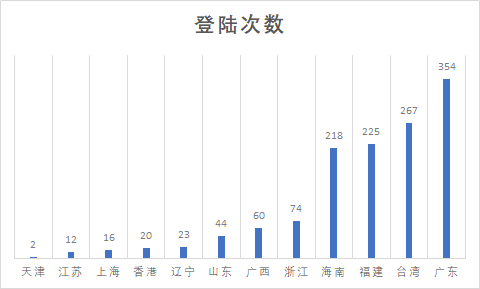
\includegraphics[width=.6\textwidth]{1949-2018_province_occurence.png}
    \caption{1949年到2018年我国沿海各省份热带气旋的登陆次数柱状图}
    \label{figure1}
\end{figure}


\section{并排图片、表格}
\begin{figure}[H]
\begin{floatrow} \CenterFloatBoxes
    \ffigbox{\caption{2}}{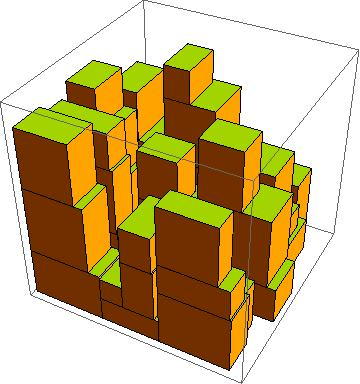
\includegraphics[width=.3\textwidth]{2.jpg}}
    \killfloatstyle
    \ttabbox{\caption{3}}{
    \begin{tabular}{|m{0.1\textwidth}<{\centering}|m{0.1\textwidth}<{\centering}|m{0.1\textwidth}<{\centering}|}\hline
        a & b & c \\ \hline
        1 & 2 & 3 \\ \hline
    \end{tabular}}
\end{floatrow}
\caption{3}
\end{figure}

\begin{figure}[H]
    \begin{floatrow}
    \ffigbox{\caption{1}}{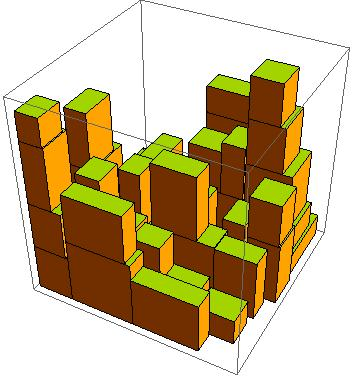
\includegraphics[width=.3\textwidth]{1.jpg}}
    \ffigbox{\caption{2}}{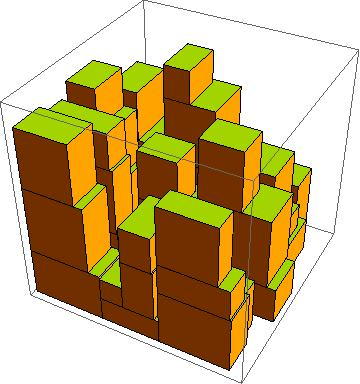
\includegraphics[width=.3\textwidth]{2.jpg}}
\end{floatrow}
\end{figure}

\section{数学公式}
\begin{equation}
    \sum\limits_{n=1}^Na_n
\end{equation}


\begin{equation}
    \begin{matrix} 
        r_{11}  &&    \cdots  &&  r_{1n}  \\
        r_{21}  &&  \cdots  &&  r_{2n}    \\ 
        \cdots  &&  \cdots  &&  \cdots    \\
        r_{81}  &&  \cdots  &&  r_{8n}    \\ 
    \end{matrix} 
    \quad\quad
    \begin{pmatrix} 
        r_{11}  &&  \cdots  &&  r_{1n}  \\
        r_{21}  &&  \cdots  &&  r_{2n}  \\ 
        \cdots  &&  \cdots  &&  \cdots  \\
        r_{81}  &&  \cdots  &&  r_{8n}  \\ 
    \end{pmatrix} 
    \quad\quad
    \begin{bmatrix} 
        r_{11}  &&  \cdots  &&  r_{1n}  \\
        r_{21}  &&  \cdots  &&  r_{2n}  \\ 
        \cdots  &&  \cdots  &&  \cdots  \\
        r_{81}  &&  \cdots  &&  r_{8n}  
    \end{bmatrix} 
\end{equation}

\begin{equation}
    \begin{Bmatrix} 
        r_{11}  &&  \cdots  &&  r_{1n}  \\
        r_{21}  &&  \cdots  &&  r_{2n}  \\ 
        \cdots  &&  \cdots  &&  \cdots  \\
        r_{81}  &&  \cdots  &&  r_{8n}  \\
    \end{Bmatrix} 
    \quad\quad
    \begin{vmatrix} 
        r_{11}  &&  \cdots  &&  r_{1n}  \\
        r_{21}  &&  \cdots  &&  r_{2n}  \\ 
        \cdots  &&  \cdots  &&  \cdots  \\
        r_{81}  &&  \cdots  &&  r_{8n}  \\
    \end{vmatrix} 
    \quad\quad
    \begin{Vmatrix} 
        r_{11}  &&  \cdots  &&  r_{1n}  \\
        r_{21}  &&  \cdots  &&  r_{2n}  \\ 
        \cdots  &&  \cdots  &&  \cdots  \\
        r_{81}  &&  \cdots  &&  r_{8n}  
    \end{Vmatrix}     
\end{equation}



\end{appendices}
\end{document} 
